\documentclass[letterpaper,12pt]{article}

%\usepackage{amsmath}
\usepackage{comment}
\RequirePackage[hypertex]{hyperref}
    \hypersetup{colorlinks=true,urlcolor=blue,linkcolor=red}
\RequirePackage{GE05}

\newcommand{\GDP}{\mbox{\em GDP\/}}
\newcommand{\NDP}{\mbox{\em NDP\/}}
\newcommand{\GNP}{\mbox{\em GNP\/}}
\newcommand{\NX}{\mbox{\em NX\/}}
\newcommand{\NY}{\mbox{\em NY\/}}
\newcommand{\CA}{\mbox{\em CA\/}}
\newcommand{\NFA}{\mbox{\em NFA\/}}
\newcommand{\Def}{\mbox{\em Def\/}}
\newcommand{\CPI}{\mbox{\em CPI\/}}

\def\ClassName{The Global Economy}
\def\Category{Class Notes}
\def\HeadName{Business Cycle Properties}

\begin{document}
\thispagestyle{empty}%
\Head

\centerline{\large \bf \HeadName}%
\centerline{Revised: \today}

\bigskip
Over the last two centuries, US real GDP has grown at an average
rate between 3 and 3.5\% a year, 
but this growth has been anything but smooth:  
annual growth rates over the last fifty years have
ranged from $-2$\% (in 1975 and 1982) to 8\% (1966 and 1985). 
These short-term fluctuations or business cycles 
are the subject of intense interest by businesses  
and play an important role in their decisions to hire, produce, and invest. 
And it's not just the US; 
although we will use US data, other economies exhibit similar
volatility.  
Emerging markets, including the US in the 19th century, 
differ primarily in having greater volatility.  
The bottom line:  fluctuations in economic growth 
are a fact of life.  

Our mission is to outline some of the basic features 
of these fluctuations, which point to ways of dealing with 
the inevitable risk and uncertainty they bring to our economic lives.  


\begin{figure}[h]
    \centering
    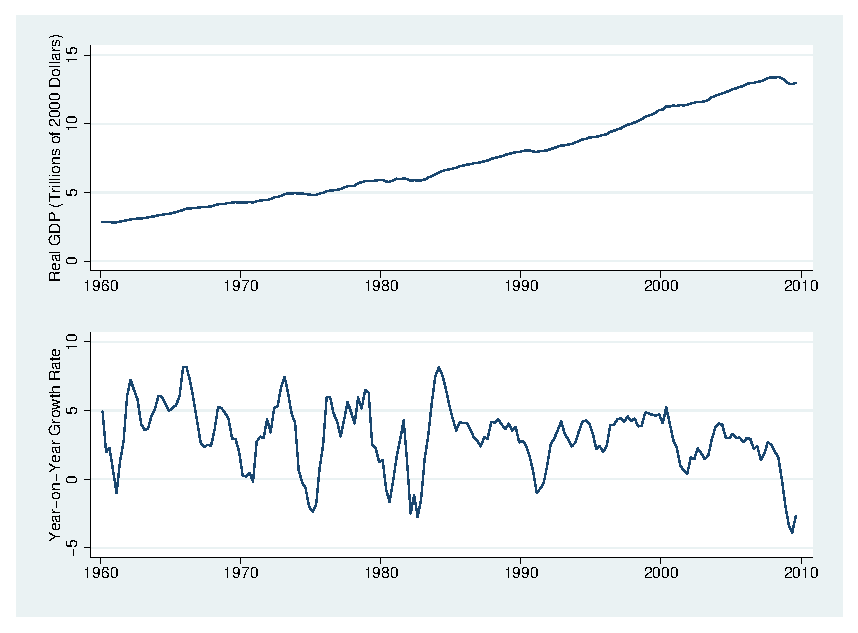
\includegraphics[scale=0.8]{usygy.eps}
    \caption{Level and Fluctuations of US Real GDP.}
    \label{fig:yandgy}
\end{figure}


\subsubsection*{Fluctuations in GDP growth}

You can get a sense of these economy-wide fluctuations 
from Figure~\ref{fig:yandgy}, 
where we plot real GDP and its year-on-year growth rate --- 
the rate of growth of quarterly GDP over the same quarter a year earlier.
%
%\begin{figure}[h]
%    \centering
%    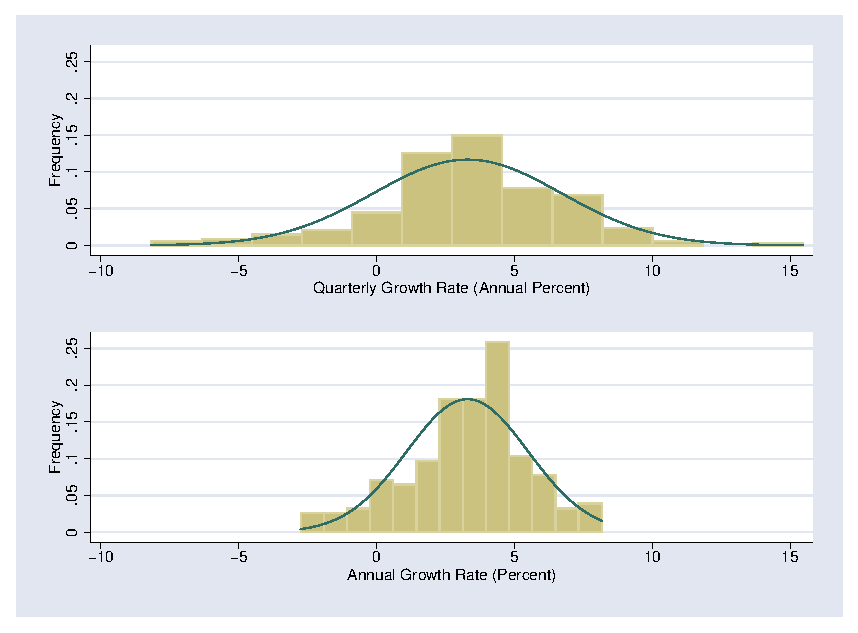
\includegraphics[scale=0.80]{ushist.eps}
%    \caption{Histogram of Fluctuations in US Real GDP.}
%    \label{fig:histogram}%
%\end{figure}
%
Volatility is obvious in the wide range of growth rates.
The figure also suggests that volatility was lower between 1985 
and 2008.   
Whether this ``great moderation'' is now in the past remains to be seen.  
Experience tells us, however, 
that periodic reports of the death of the business cycle
have yet to pan out.  



\subsubsection*{Expenditure components}

%These recurring fluctuations follow some regular patterns. 
Arthur Burns and Wesley Mitchell, two pioneers of business cycle research, 
wrote in 1946:  
%
\begin{quote} 
{Business cycles are a type of
fluctuation found in the aggregate economic activity of
nations.... A cycle consists of expansions occurring at about the
same time in many economic activities, followed by similarly
general recessions, contractions and revivals which merge into the
expansion phases of the next cycle; this sequence of changes is
recurrent but not periodic; in duration business cycles vary from
more than one year to ten or twelve years.}
%(From: {\it Measuring Business Cycles\/}, NBER, 1946.)
\end{quote}
%
Burns and Mitchell refer to fluctuations in 
``many economic activities.'' 
Among these activities are the expenditure
components of GDP.   
Are their fluctuations similar to those of GDP?
On the whole, the components, particularly consumption and investment, 
move up and down together, although the magnitudes vary.  
%Table~\ref{tab:cycleprops} and 
%Figure \ref{fig:expenditure_components} document 
%these tendencies for the US.

\begin{table}[h]
\begin{center}
\begin{tabular}{lccc}
\hline
        &  Std Dev (\%)  &  Corr w/ GDP  \\
\hline                 
GDP     &      2.19          &    1.00      \\
Consumption:  total      &  1.75  &  0.84   \\
Consumption:  services   &  1.22  &  0.63   \\
Consumption:  nondurable &  1.65  &  0.75   \\
Consumption:  durables   &  6.29  &  0.76   \\
Investment:  total       &  6.64  &  0.86   \\
Investment:  structures  &  7.85  &  0.46   \\
Investment:  equipment   &  7.35  &  0.81   \\
Investment:  housing     &  13.05\phantom{1} &  0.60   \\
Employment               &  1.77  &  0.76   \\
S\&P 500 Index           &  14.98\phantom{1}  &  0.36   \\
\hline 
\end{tabular}
\caption{Properties of Growth Rates.
Numbers refer to year-on-year growth rates 
computed from quarterly US data.}
\label{tab:cycleprops}
\end{center}
\end{table}


\begin{figure}[h]
    \centering
    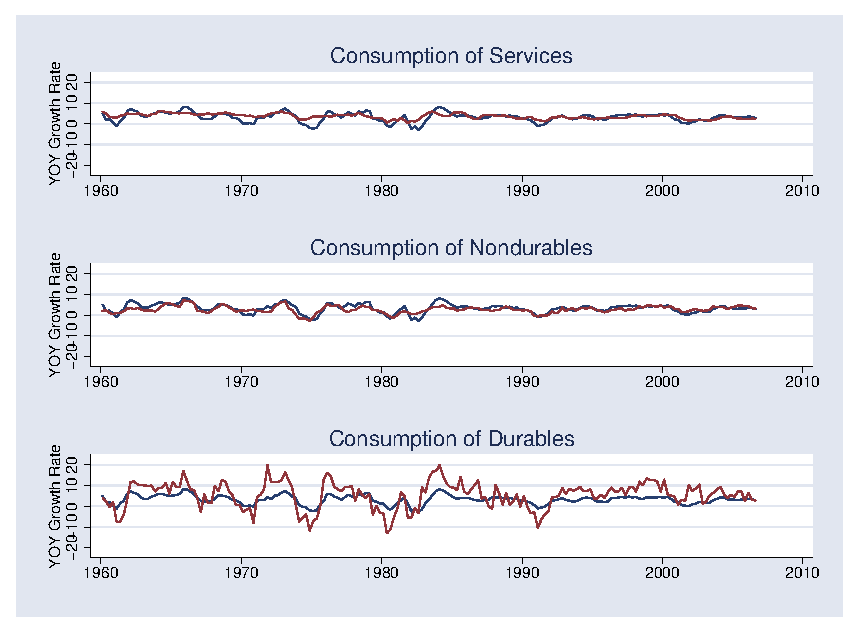
\includegraphics[scale=0.8]{usgcall.eps}
    \caption{Fluctuations in Consumption and GDP.
    The solid (blue) line is real GDP, the other (red) line
    a component of consumption.}
    \label{fig:gcall}%
\end{figure}

\begin{figure}[h]
    \centering
    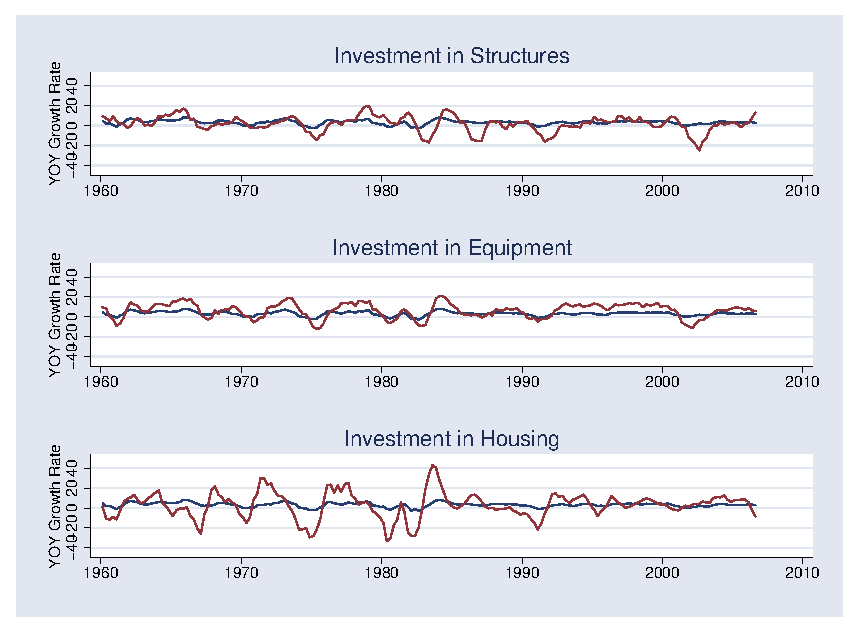
\includegraphics[scale=0.8]{usgiall.eps}
    \caption{Fluctuations in Investment and GDP.
    The solid (blue) line is real GDP, the other (red) line
    a component of investment.}
    \label{fig:giall}%
\end{figure}


Consumption currently accounts for about 70\% of US GDP;  
as you might expect, its fluctuations are similar.
The correlation of year-on-year growth rates in consumption (total) 
and GDP is 0.84; see Table~\ref{tab:cycleprops}.
Its major components --- services, nondurable goods, 
and durable goods --- also vary with GDP, 
but their correlations and (esp) volatilities differ somewhat.
Consumption of nondurables and services 
is less volatile than GDP, in the sense that 
the standard deviation of its growth rate is smaller.
You can see this clearly in Figure~\ref{fig:gcall}.
The dark line in each panel is GDP, 
the other line a component of consumption.
It's apparent that consumption of durables is far more
volatile than consumption of nondurables and services.
You might think of specific products and industries that reflect
the same phenomenon.
Why do you think cars and refrigerators 
are more volatile than haircuts and medical care?  


Investment (new plant and equipment) also moves up and down with output, 
and is substantially more volatile.  
As a rule of thumb, a 1\% increase in GDP is associated with 
about a 3\% increase in total investment.  
(We're looking at the ratio of standard deviations here, 
and the high correlation of the two series.) 
Table~\ref{tab:cycleprops} and Figure~\ref{fig:giall} 
show that the major components --- structures, equipment, 
and residential housing --- are highly correlated with, 
and more volatile than, GDP.  


When we turn to business cycle indicators, we'll see that 
many of them are more detailed measures of 
some aspect of consumption or investment.
Consumption is important, because it accounts for most of GDP.
Investment is important, because it is highly responsive
to changes in economic conditions.  


\subsubsection*{Labor and capital markets}


If the expenditure components of GDP move up and down together, 
so, too, do labor and capital markets.  
Employment, for example, varies directly with GDP: 
the correlation between their growth rates is 0.76.
We see in Figure~\ref{fig:gother} that 
employment growth is generally less than GDP growth;  
the difference reflects an increase in output per worker, 
a good thing, to be sure!

Aggregate stock prices are extremely volatile, with a standard deviation
about eight times larger than GDP.
The correlation with GDP (0.36) suggests that 
good news about the economy is good news for stock prices.  
We'll see later that stock prices lead GDP:
the correlation of stock prices with GDP two quarters later is above 0.5.
We'll look at this more closely when we turn to indicators.  

%
\begin{figure}
    \centering
    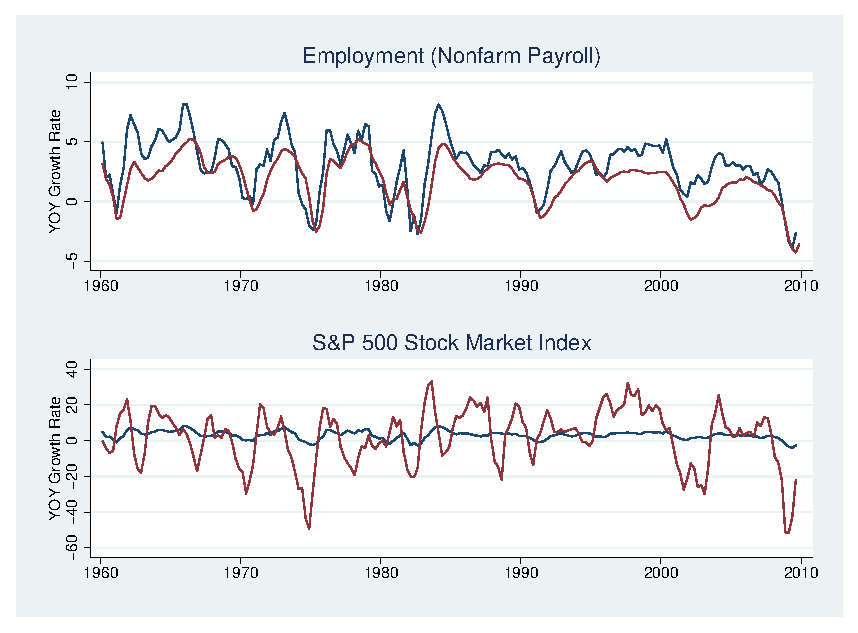
\includegraphics[scale=0.8]{usgother.eps}
    \caption{Fluctuations in Employment and Stock Prices. 
    The solid (blue) line is real GDP, the other (red) line 
    employment (top panel) or the S\&P 500 Index (bottom).} 
    \label{fig:gother}%
\end{figure}


\subsubsection*{Executive summary}

\begin{enumerate}
\item Economic growth varies over time, 
even in relatively stable developed countries like the US.  

\item Lots of things move up and down together:  
consumption, investment, and employment typically move up and down
with GDP.  

\item Purchases (and production) of durable goods vary more 
than purchases of nondurable goods and services. 
Here durable goods includes both consumer durables 
(cars, for example) and producer durables 
(plant and equipment).  

\end{enumerate}


\begin{comment}
\subsubsection*{Review questions}

Think about each of the following questions, which we'll address
at greater length shortly.
%
\begin{enumerate}

\item Why is consumption is less volatile than output? Investment
more volatile?

\item Why does employment lag output?

\item Why does the stock market lead output?

\item Why does the yield curve steepen before an expansion?

\end{enumerate}
\end{comment}

\subsubsection*{Further reading}

The Burns and Mitchell quotation is from their 
{\it Measuring Business Cycles\/}, NBER, 1946.


%For more information:
%
%\begin{itemize}
%\item National Bureau of Economic Research: US
%\href{http://www.nber.org/cycles.html/}{business cycle dates} and
%\href{http://www.nber.org/releases/}{calendar} of release dates
%for international economic indicators (you can sign up for free
%email reminders).
%\end{itemize}


\vfill \centerline{\it \copyright \ \number\year \ NYU Stern
School of Business}

\end{document}
